%%
% This is an Overleaf template for presentations
% using the TUM Corporate Desing https://www.tum.de/cd
%
% For further details on how to use the template, take a look at our
% GitLab repository and browse through our test documents
% https://gitlab.lrz.de/latex4ei/tum-templates.
%
% The tumbeamer class is based on the beamer class.
% If you need further customization please consult the beamer class guide
% https://ctan.org/pkg/beamer.
% Additional class options are passed down to the base class.
%
% If you encounter any bugs or undesired behaviour, please raise an issue
% in our GitLab repository
% https://gitlab.lrz.de/latex4ei/tum-templates/issues
% and provide a description and minimal working example of your problem.
%%

\PassOptionsToClass{onlytextwidth}{beamer}

\documentclass[
  german,            % define the document language (english, german)
  aspectratio=169,    % define the aspect ratio (169, 43)
  % handout=2on1,       % create handout with multiple slides (2on1, 4on1)
  % partpage=false,     % insert page at beginning of parts (true, false)
  % sectionpage=true,   % insert page at beginning of sections (true, false)
]{tumbeamer}


% load additional packages
\usepackage{booktabs}
\usepackage{graphicx}
\usepackage{tikz}
\usepackage{url}
\usepackage{pgf}
\usepackage{pgfplots}
\usepackage{hyperref}
\usepackage{pmboxdraw}
\usepackage{float}
\usepackage{babel}[ngerman]
\usepackage{csquotes}[autostyle]
\usepackage[useregional]{datetime2}
\usepackage[cache=true]{minted}
\usemintedstyle{borland}
\usepackage{listings}
\usepackage{amsmath}
\usepackage{xcolor}

% tikz  
\usetikzlibrary{fit, matrix, calc, arrows, arrows.meta, positioning, patterns, patterns.meta, bending, overlay-beamer-styles, shapes, shapes.geometric, shapes.misc, backgrounds}

% https://tex.stackexchange.com/a/7045
\newcommand*\circled[1]{\tikz[baseline=(char.base)]{
		\node[shape=circle,draw,inner sep=2pt, font=\scriptsize] (char) {#1};}}

\newcommand*\colorcirc[1]{\tikz[baseline=(char.base)]{
		\node[shape=circle,fill=#1,inner sep=2pt] {};}}

% minted
\setminted{
    fontsize=\small, 
    frame=none,
    breaklines=true,
}

\captionsetup{labelformat=empty}

% image path
\graphicspath{ {./resources/} }

% beamer
\setbeamercolor{footnote}{fg=black}
\setbeamercolor{footnote mark}{fg=black}
\renewcommand{\thempfootnote}{\arabic{mpfootnote}}

% presentation metadata
\title{Übung 05: Caches}
\subtitle{Einführung in die Rechnerarchitektur}
\author{Niklas Ladurner}

\institute{\theChairName\\\theDepartmentName\\\theUniversityName}
\date{\DTMdisplaydate{2025}{11}{14}{-1}}

\footline{\insertauthor~|~\insertshorttitle~|~\insertshortdate}


% macro to configure the style of the presentation
\TUMbeamersetup{
  title page = TUM tower,         % style of the title page
  part page = TUM toc,            % style of part pages
  section page = TUM toc,         % style of section pages
  content page = TUM more space,  % style of normal content pages
  tower scale = 1.0,              % scaling factor of TUM tower (if used)
  headline = TUM threeliner,      % which variation of headline to use
  footline = TUM default,         % which variation of footline to use
  % configure on which pages headlines and footlines should be printed
  headline on = {title page},
  footline on = {every page, title page=false},
}

\begin{document}

\maketitle

\begin{frame}[c, fragile]{}{}
	\begin{center}
		\LARGE  Keine Garantie für die Richtigkeit der Tutorfolien.

		\Large Bei Unklarheiten/Unstimmigkeiten haben VL/ZÜ-Folien recht!
	\end{center}
\end{frame}

\begin{frame}[fragile, c]{Motivation}{}
	\begin{itemize}
		\item Zugriffe auf Hauptspeicher ($\equiv$ RAM) sind \textbf{extrem} langsam. Lösung: Caches
		\item \enquote{Zwischenstation} zwischen Registern (sehr schnell, sehr klein) und Hauptspeicher (sehr langsam, sehr groß)
		\item Idee: Häufig genutzte Daten im Cache zwischenspeichern, der Rest wird bei Bedarf aus dem Hauptspeicher geholt
		\item Die Position eines Datums im Cache wird durch die Adresse des Zugriffs bestimmt
		\item Heutzutage meist L1/L2/L3-Caches: Caches aufsteigender Größe, aber absteigender Zugriffszeit
	\end{itemize}
\end{frame}


\begin{frame}[t]{Terminologie}
	\vspace*{1cm}
	\begin{itemize}
		\item \textbf{Hit}: Datum liegt im Cache
		\item \textbf{Miss}: Datum nicht im Cache, muss erst aus Hauptspeicher geholt werden\\$\rightarrow$ Ziel: möglichst hohe \textbf{Hitrate} (Hits/Anfragen), d.h. häufig genutzte Daten im Cache

	\end{itemize}
	\vfill{}
	\pause
	\begin{itemize}
		\item \textbf{zeitliche} Lokalität\only<2>{\footnote{Definition der Lokalitätsprinzipien ist eine beliebte Klausuraufgabe!}}: Zugriff auf $x$ $\rightarrow$ Zugriff auf $x$ in Zukunft wahrscheinlicher
		\item \textbf{räumliche} Lokalität: Zugriff auf $x$ $\rightarrow$ Zugriff auf Daten in der Nähe wahrscheinlicher\\$\rightarrow$ Konsequenz: Cachen von ganzer Cachezeile
	\end{itemize}
\end{frame}

\begin{frame}[c]{Direktabbildender Cache\footnote{Englisch: Direct Mapped Cache}}
	\begin{columns}[c]
		\begin{column}{0.5\textwidth}
			\only<1-3>{
				\begin{itemize}
					\item direkte (surjektive) Abbildung von\\Hauptspeicheradresse $\mapsto$ Cacheadresse
					\item jedes Datum aus dem Hauptspeicher kann nur in \textit{eine} bestimmte Cachezeile gecached werden
					\item <2->Beispiel: 16-Bit-Architektur, 8 Cachezeilen zu je 4 Byte
					      \begin{enumerate}
						      \item Anzahl Offset-Bits:  \visible<3->{$\log_2(4)=2$}
						      \item Anzahl Index-Bits: \visible<3->{$\log_2(8)=3$}
						      \item Anzahl Tag-Bits: \visible<3->{$16-3-2=11$}
					      \end{enumerate}
				\end{itemize}
			}
			\only<4->{
				\begin{center}
					\resizebox{\textwidth}{!}{
						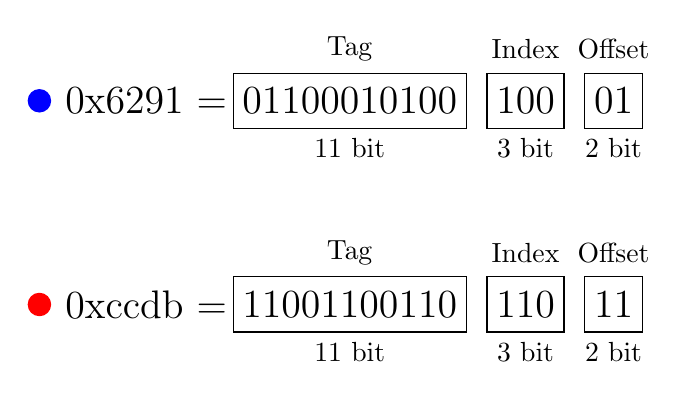
\begin{tikzpicture}
							\node[draw=none] (addr) {\Large\textrm{0x6291} $=$};
							\node[shape=circle,fill=blue,inner sep=3pt, left=0.05cm of addr] {};

							\matrix[matrix of nodes, ampersand replacement=\&, nodes={draw, minimum width=0.5cm, minimum height=0.7cm, anchor=center}, column sep=0.25cm, font={\Large}, right=-0.5em of addr.east] (mat) {
								{$01100010100$} \& {$100$} \& {$01$} \\
							};
							\node[above=0.3cm of mat-1-1.north, anchor=center] {\textrm{Tag}};
							\node[above=0.3cm of mat-1-2.north, anchor=center] {\textrm{Index}};
							\node[above=0.3cm of mat-1-3.north, anchor=center] {\textrm{Offset}};

							\node[below=0cm of mat-1-1.south, anchor=north] {\textrm{11 bit}};
							\node[below=0cm of mat-1-2.south, anchor=north] {\textrm{3 bit}};
							\node[below=0cm of mat-1-3.south, anchor=north] {\textrm{2 bit}};

							\visible<5->{
								\node[draw=none, below=2cm of addr] (addr2) {\Large\textrm{0xccdb} $=$};
								\node[shape=circle,fill=red,inner sep=3pt, left=0.05cm of addr2] {};

								\matrix[matrix of nodes, ampersand replacement=\&, nodes={draw, minimum width=0.5cm, minimum height=0.7cm, anchor=center}, column sep=0.25cm, font={\Large}, right=-0.5em of addr2.east] (mat2) {
									{$11001100110$} \& {$110$} \& {$11$} \\
								};
								\node[above=0.3cm of mat2-1-1.north, anchor=center] {\textrm{Tag}};
								\node[above=0.3cm of mat2-1-2.north, anchor=center] {\textrm{Index}};
								\node[above=0.3cm of mat2-1-3.north, anchor=center] {\textrm{Offset}};

								\node[below=0cm of mat2-1-1.south, anchor=north] {\textrm{11 bit}};
								\node[below=0cm of mat2-1-2.south, anchor=north] {\textrm{3 bit}};
								\node[below=0cm of mat2-1-3.south, anchor=north] {\textrm{2 bit}};
							}
						\end{tikzpicture}
					}
					\scriptsize Es wird immer die gesamte Cachezeile ausgetauscht!
				\end{center}
			}
		\end{column}%
		\begin{column}{0.5\textwidth}
			\visible<2->{
				\vspace*{-1cm}
				\begin{center}
					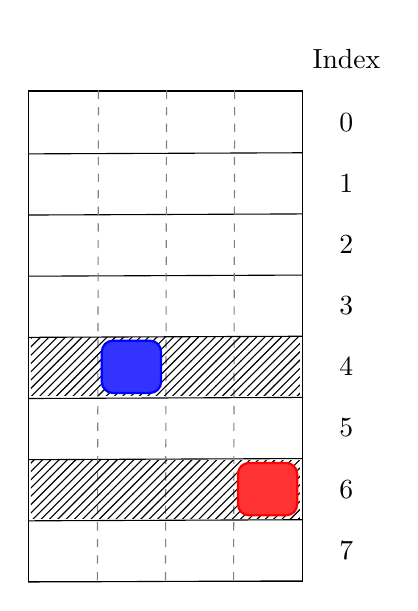
\begin{tikzpicture}
						\def\cellht{2.25em}
						\def\cellwt{2.5em}

						\tikzset{
							label/.style = {draw=none, minimum height=\cellht},
							biglabel/.style = {text width=2cm, align=center, anchor=west},
							arrow/.style={Latex-, thick},
							matstyle/.style={matrix of nodes, draw,ampersand replacement=\&, nodes={draw=none, minimum width=\cellwt, minimum height=\cellht, text height=1em, text depth=0.25em, align=center}, column sep=-\pgflinewidth, row sep=-\pgflinewidth, anchor=north west, inner sep=0pt},
							bbrace/.style={decorate,decoration={brace,amplitude=5pt,raise=0.5em}, rotate=90, thick},
							bbox/.style={fill=blue!80, draw=blue, rounded corners, thick, inner sep=-2pt},
							bbox2/.style={red, pattern=north east lines, inner sep=-1pt},
							tag/.style={black,fill=black, minimum width=0.75em, minimum height=0.75em, inner sep=0pt},
						}

						\matrix[matstyle] (mat) at (0, 0) {
						{}\&{}\&{}\&{}%
						\\{}\&{}\&{}\&{}%
						\\{}\&{}\&{}\&{}%
						\\{}\&{}\&{}\&{}%
						\\{}\&{}\&{}\&{}%
						\\{}\&{}\&{}\&{}%
						\\{}\&{}\&{}\&{}%
						\\{}\&{}\&{}\&{}\\
						};

						%						\node[label, below=0cm of mat.south] (tinfo) {gespeichertes Tag};
						%						\node[tag, left=0cm of tinfo, yshift=0.1em] {};

						\node[label, anchor=south west] (ilabel) at (mat-1-4.north east) {Index};

						\foreach[count=\i from 0] \y in {1,...,8}{
								\draw (mat-\y-1.south west) -- ($(mat-\y-4.south east) + (0, \pgflinewidth)$);
								\node[label] at (mat-\y-4.east -|  ilabel) {\i};
							}
						\foreach \x in {1,2,3}{
								\draw[dashed, thin, gray] (mat-1-\x.north east) -- ($(mat-8-\x.south east) - (\pgflinewidth, 0)$);
							}

						\node[bbox2, visible on=<4>, fit=(mat-5-1.north west) (mat-5-4.south east)] {};
						\node[bbox, visible on=<4->, fit=(mat-5-2.north west) (mat-5-2.south east)] {};
						%						\node[tag, visible on=<4->, left=1.2cm of mat-4-1.east] {};

						\node[bbox2, visible on=<5>, fit=(mat-7-1.north west) (mat-7-4.south east)] {};
						\node[bbox, fill=red!80, draw=red,visible on=<5->, fit=(mat-7-4.north west) (mat-7-4.south east)] {};
						%						\node[tag, visible on=<5->, left=1.2cm of mat-7-1.east] {};
					\end{tikzpicture}
				\end{center}
			}
		\end{column}
	\end{columns}
\end{frame}

\begin{frame}[c]{Vollassoziativer Cache\footnote{Englisch: Fully Associative Cache}}
	\begin{columns}[c]
		\begin{column}{0.5\textwidth}
			\only<1-3>{
				\begin{itemize}
					\item Daten werden \enquote{wo gerade Platz ist} gecached
					\item jedes Datum aus dem Hauptspeicher kann in eine \textit{beliebige} Cachezeile gecached werden
					\item <2->Beispiel: 16-Bit-Architektur, 8 Cachezeilen zu je 4 Byte
					      \begin{enumerate}
						      \item Anzahl Offset-Bits:  \visible<3->{$\log_2(4)=2$}
						      \item Anzahl Index-Bits: \visible<3->{$0$}
						      \item Anzahl Tag-Bits: \visible<3->{$16-2-0=14$}
					      \end{enumerate}
				\end{itemize}
			}
			\only<4->{
				\begin{center}
					\resizebox{\textwidth}{!}{
						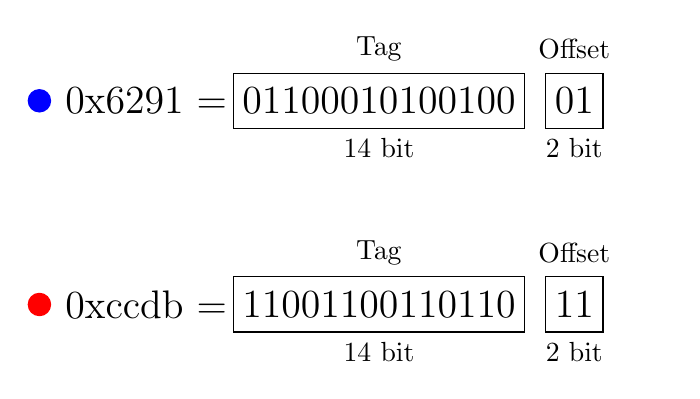
\begin{tikzpicture}
							\node[draw=none] (addr) {\Large\textrm{0x6291} $=$};
							\node[shape=circle,fill=blue,inner sep=3pt, left=0.05cm of addr] {};

							\matrix[matrix of nodes, ampersand replacement=\&, nodes={draw, minimum width=0.5cm, minimum height=0.7cm, anchor=center}, column sep=0.25cm, font={\Large}, right=-0.5em of addr.east] (mat) {
							{$01100010100100$} \& {$01$} \& |[draw=none]| {}\\
							};
							\node[above=0.3cm of mat-1-1.north, anchor=center] {\textrm{Tag}};
							\node[above=0.3cm of mat-1-2.north, anchor=center] {\textrm{Offset}};

							\node[below=0cm of mat-1-1.south, anchor=north] {\textrm{14 bit}};
							\node[below=0cm of mat-1-2.south, anchor=north] {\textrm{2 bit}};

							\visible<5->{
								\node[draw=none, below=2cm of addr] (addr2) {\Large\textrm{0xccdb} $=$};
								\node[shape=circle,fill=red,inner sep=3pt, left=0.05cm of addr2] {};

								\matrix[matrix of nodes, ampersand replacement=\&, nodes={draw, minimum width=0.5cm, minimum height=0.7cm, anchor=center}, column sep=0.25cm, font={\Large}, right=-0.5em of addr2.east] (mat2) {
									{$11001100110110$} \& {$11$} \\
								};
								\node[above=0.3cm of mat2-1-1.north, anchor=center] {\textrm{Tag}};
								\node[above=0.3cm of mat2-1-2.north, anchor=center] {\textrm{Offset}};

								\node[below=0cm of mat2-1-1.south, anchor=north] {\textrm{14 bit}};
								\node[below=0cm of mat2-1-2.south, anchor=north] {\textrm{2 bit}};
							}
						\end{tikzpicture}
					}
					\scriptsize Es wird immer die gesamte Cachezeile ausgetauscht!
				\end{center}
			}
		\end{column}%
		\begin{column}{0.5\textwidth}
			\visible<2->{
				\vspace*{-1cm}
				\begin{center}
					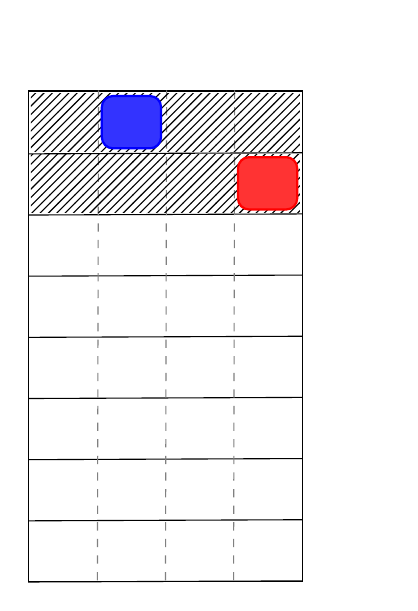
\begin{tikzpicture}
						\def\cellht{2.25em}
						\def\cellwt{2.5em}

						\tikzset{
							label/.style = {draw=none, minimum height=\cellht},
							biglabel/.style = {text width=2cm, align=center, anchor=west},
							arrow/.style={Latex-, thick},
							matstyle/.style={matrix of nodes, draw,ampersand replacement=\&, nodes={draw=none, minimum width=\cellwt, minimum height=\cellht, text height=1em, text depth=0.25em, align=center}, column sep=-\pgflinewidth, row sep=-\pgflinewidth, anchor=north west, inner sep=0pt},
							bbrace/.style={decorate,decoration={brace,amplitude=5pt,raise=0.5em}, rotate=90, thick},
							bbox/.style={fill=blue!80, draw=blue, rounded corners, thick, inner sep=-2pt},
							bbox2/.style={red, pattern=north east lines, inner sep=-1pt},
						}

						\matrix[matstyle] (mat) at (0, 0) {
						{}\&{}\&{}\&{}%
						\\{}\&{}\&{}\&{}%
						\\{}\&{}\&{}\&{}%
						\\{}\&{}\&{}\&{}%
						\\{}\&{}\&{}\&{}%
						\\{}\&{}\&{}\&{}%
						\\{}\&{}\&{}\&{}%
						\\{}\&{}\&{}\&{}\\
						};

						\node[label, anchor=south west] (ilabel) at (mat-1-4.north east) {\phantom{Index}};

						\foreach[count=\i from 0] \y in {1,...,8}{
								\draw (mat-\y-1.south west) -- ($(mat-\y-4.south east) + (0, \pgflinewidth)$);
								\node[label] at (mat-\y-4.east -|  ilabel) {\phantom{\i}};
							}
						\foreach \x in {1,2,3}{
								\draw[dashed, thin, gray] (mat-1-\x.north east) -- ($(mat-8-\x.south east) - (\pgflinewidth, 0)$);
							}

						\node[bbox2, visible on=<4>, fit=(mat-1-1.north west) (mat-1-4.south east)] {};
						\node[bbox, visible on=<4->, fit=(mat-1-2.north west) (mat-1-2.south east)] {};

						\node[bbox2, visible on=<5>, fit=(mat-2-1.north west) (mat-2-4.south east)] {};
						\node[bbox, fill=red!80, draw=red,visible on=<5->, fit=(mat-2-4.north west) (mat-2-4.south east)] {};
					\end{tikzpicture}
				\end{center}
			}
		\end{column}
	\end{columns}
\end{frame}

\begin{frame}[c]{Mengenassoziativer Cache\footnote{Englisch: Set Associative Cache}}
	\begin{columns}[c]
		\begin{column}{0.5\textwidth}
			\only<1-3>{
				\begin{itemize}
					\item Aufteilung des Cache in Sets zu je $n$ Cachezeilen
					\item jedes Datum aus dem Hauptspeicher kann nur in \textit{einem} bestimmtem Set gecached werden, im Set aber in einer \textit{beliebigen} Cachezeile stehen
					\item <2->Beispiel: 16-Bit-Architektur, 8 Cachezeilen zu je 4 Byte, 2-fach assoziativ
					      \begin{enumerate}
						      \item Anzahl Cache-Sets:  \visible<3->{$\frac{8}{2}=4$}
						      \item Anzahl Offset-Bits:  \visible<3->{$\log_2(4)=2$}
						      \item Anzahl Index-Bits: \visible<3->{$\log_2(4)=2$}
						      \item Anzahl Tag-Bits: \visible<3->{$16-2-2=12$}
					      \end{enumerate}
				\end{itemize}
			}
			\only<4->{
				\begin{center}
					\resizebox{\textwidth}{!}{
						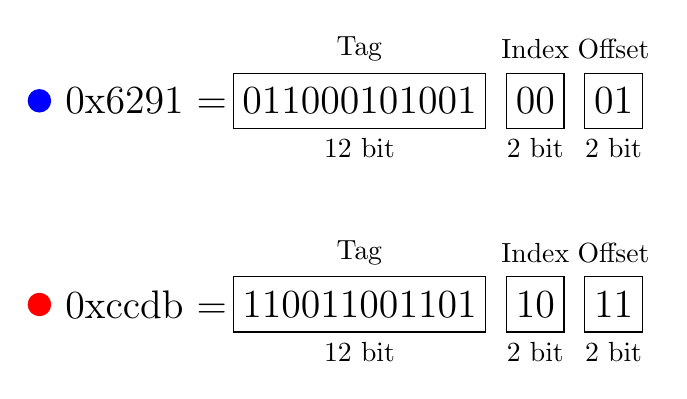
\begin{tikzpicture}
							\node[draw=none] (addr) {\Large\textrm{0x6291} $=$};
							\node[shape=circle,fill=blue,inner sep=3pt, left=0.05cm of addr] {};

							\matrix[matrix of nodes, ampersand replacement=\&, nodes={draw, minimum width=0.5cm, minimum height=0.7cm, anchor=center}, column sep=0.25cm, font={\Large}, right=-0.5em of addr.east] (mat) {
								{$011000101001$} \& {$00$} \& {$01$} \\
							};
							\node[above=0.3cm of mat-1-1.north, anchor=center] {\textrm{Tag}};
							\node[above=0.3cm of mat-1-2.north, anchor=center] {\textrm{Index}};
							\node[above=0.3cm of mat-1-3.north, anchor=center] {\textrm{Offset}};

							\node[below=0cm of mat-1-1.south, anchor=north] {\textrm{12 bit}};
							\node[below=0cm of mat-1-2.south, anchor=north] {\textrm{2 bit}};
							\node[below=0cm of mat-1-3.south, anchor=north] {\textrm{2 bit}};

							\visible<5->{
								\node[draw=none, below=2cm of addr] (addr2) {\Large\textrm{0xccdb} $=$};
								\node[shape=circle,fill=red,inner sep=3pt, left=0.05cm of addr2] {};

								\matrix[matrix of nodes, ampersand replacement=\&, nodes={draw, minimum width=0.5cm, minimum height=0.7cm, anchor=center}, column sep=0.25cm, font={\Large}, right=-0.5em of addr2.east] (mat2) {
									{$110011001101$} \& {$10$} \& {$11$} \\
								};
								\node[above=0.3cm of mat2-1-1.north, anchor=center] {\textrm{Tag}};
								\node[above=0.3cm of mat2-1-2.north, anchor=center] {\textrm{Index}};
								\node[above=0.3cm of mat2-1-3.north, anchor=center] {\textrm{Offset}};

								\node[below=0cm of mat2-1-1.south, anchor=north] {\textrm{12 bit}};
								\node[below=0cm of mat2-1-2.south, anchor=north] {\textrm{2 bit}};
								\node[below=0cm of mat2-1-3.south, anchor=north] {\textrm{2 bit}};
							}
						\end{tikzpicture}
					}
					\scriptsize Es wird immer die gesamte Cachezeile ausgetauscht!
				\end{center}
			}
		\end{column}%
		\begin{column}{0.5\textwidth}
			\visible<2->{
				\vspace*{-1cm}
				\begin{center}
					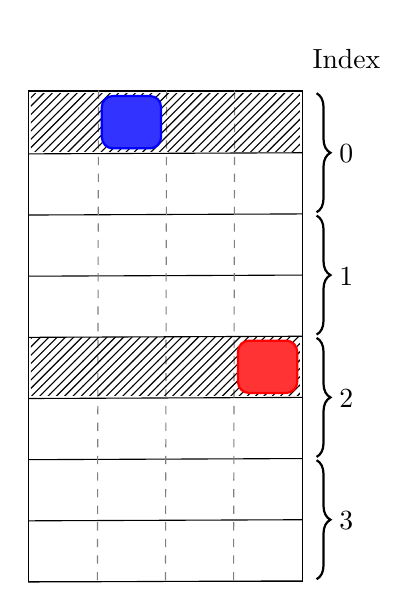
\begin{tikzpicture}
						\def\cellht{2.25em}
						\def\cellwt{2.5em}

						\tikzset{
							label/.style = {draw=none, minimum height=\cellht},
							biglabel/.style = {text width=2cm, align=center, anchor=west},
							arrow/.style={Latex-, thick},
							matstyle/.style={matrix of nodes, draw,ampersand replacement=\&, nodes={draw=none, minimum width=\cellwt, minimum height=\cellht, text height=1em, text depth=0.25em, align=center}, column sep=-\pgflinewidth, row sep=-\pgflinewidth, anchor=north west, inner sep=0pt},
							bbrace/.style={decorate,decoration={brace,amplitude=5pt,raise=0.5em}, rotate=90, thick},
							bbox/.style={fill=blue!80, draw=blue, rounded corners, thick, inner sep=-2pt},
							bbox2/.style={red, pattern=north east lines, inner sep=-1pt},
							tag/.style={black,fill=black, minimum width=0.75em, minimum height=0.75em, inner sep=0pt},
						}

						\matrix[matstyle] (mat) at (0, 0) {
						{}\&{}\&{}\&{}%
						\\{}\&{}\&{}\&{}%
						\\{}\&{}\&{}\&{}%
						\\{}\&{}\&{}\&{}%
						\\{}\&{}\&{}\&{}%
						\\{}\&{}\&{}\&{}%
						\\{}\&{}\&{}\&{}%
						\\{}\&{}\&{}\&{}\\
						};

						%						\node[label, below=0cm of mat.south] (tinfo) {gespeichertes Tag};
						%						\node[tag, left=0cm of tinfo, yshift=0.1em] {};

						\node[label, anchor=south west] (ilabel) at (mat-1-4.north east) {Index};

						\foreach \y in {1,...,8}{
								\draw (mat-\y-1.south west) -- ($(mat-\y-4.south east) + (0, \pgflinewidth)$);
							}
						\foreach \x in {1,2,3}{
								\draw[dashed, thin, gray] (mat-1-\x.north east) -- ($(mat-8-\x.south east) - (\pgflinewidth, 0)$);
							}

						\node[bbox2, visible on=<4>, fit=(mat-1-1.north west) (mat-1-4.south east)] {};
						\node[bbox, visible on=<4->, fit=(mat-1-2.north west) (mat-1-2.south east)] {};
						%						\node[tag, visible on=<4->, left=1.2cm of mat-4-1.east] {};

						\node[bbox2, visible on=<5>, fit=(mat-5-1.north west) (mat-5-4.south east)] {};
						\node[bbox, fill=red!80, draw=red,visible on=<5->, fit=(mat-5-4.north west) (mat-5-4.south east)] {};
						%						\node[tag, visible on=<5->, left=1.2cm of mat-7-1.east] {};


						\foreach \i/\a/\b in {0/1/2,1/3/4,2/5/6,3/7/8}{
								\draw [bbrace] ($(mat-\a-4.north east) + (-1pt, 0)$) -- ($(mat-\b-4.south east) + (1pt, 0)$);
								\node[label] at (mat-\a-4.south east -|  ilabel) {\i};
							}
					\end{tikzpicture}
				\end{center}
			}
		\end{column}
	\end{columns}
\end{frame}

\begin{frame}[c, fragile]{Klassifikation von Misses}
	\resizebox{\textwidth}{!}{
		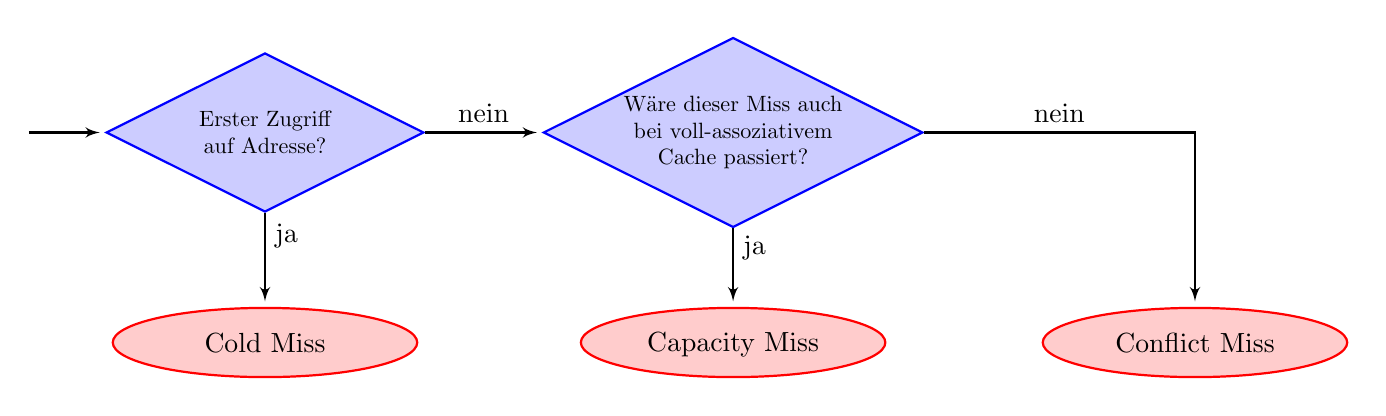
\begin{tikzpicture}
			[auto,
				ampersand replacement=\&,
				decision/.style={diamond, draw=blue, thick, fill=blue!20, text width=35mm, align=center, inner sep=1pt, scale=0.8, aspect=2},
				line/.style={draw, thick, -latex',shorten >=2pt},
				cloud/.style={draw=red, thick, ellipse,fill=red!20,
						minimum height=2.5em, text width=25mm, align=center, text depth=0pt}]

			\matrix [column sep=15mm,row sep=10mm]
			{
				\node [decision] (iscoldmiss) {Erster Zugriff auf Adresse?};
				\& \node [decision] (iscapmiss) {Wäre dieser Miss auch bei voll-assoziativem Cache passiert?}; \& \\
				\node [cloud] (coldmiss) {Cold Miss};
				\& \node [cloud] (capacitymiss) {Capacity Miss};
				\& \node [cloud] (conflictmiss) {Conflict Miss};                                                  \\
			};
			\begin{scope}[every path/.style=line]
				\path (iscoldmiss) + (left:30mm) -- (iscoldmiss);
				\path (iscoldmiss) -- node [near start] {ja} (coldmiss);
				\path (iscoldmiss) -- node [midway] {nein} (iscapmiss);
				\path (iscapmiss)  -- node [near start] {ja} (capacitymiss);
				\path (iscapmiss)  -| node [near start] {nein} (conflictmiss);
			\end{scope}
		\end{tikzpicture}}
	\vfill
	\begin{center}
		\scriptsize Nach Gschoßmann et al., 2023
	\end{center}
\end{frame}

\begin{frame}[c, fragile]{}{}
	\begin{center}
		\LARGE Fragen?
	\end{center}
\end{frame}

\begin{frame}[c, fragile]{Links}{}
	\begin{itemize}
		\item Zulip: \href{https://zulip.in.tum.de/#narrow/channel/3255-ERA-Tutorium-.E2.80.93-Mi-1600-3}{\enquote{ERA Tutorium -- Mi-1600-3}}
		      bzw. \href{https://zulip.in.tum.de/#narrow/channel/3264-ERA-Tutorium-.E2.80.93-Fr-1500-1}{\enquote{ERA Tutorium -- Fr-1500-1}}
		\item \href{https://www.moodle.tum.de/course/view.php?id=111440}{ERA-Moodle-Kurs}
		\item \href{https://artemis.tum.de/courses/516}{ERA-Artemis-Kurs}
		\item \href{https://en.wikipedia.org/wiki/Cache_placement_policies}{Wikipedia zu Caches}
		\item \href{https://www.elektronik-kompendium.de/sites/com/0309291.htm}{Elektronik-Kompendium zu Caches}
	\end{itemize}
\end{frame}

\maketitle

\end{document}
